\section{Anexo: Banco de Ejercicios Resueltos de Certámenes Pasados (2020--2025)}\markright{Anexo: Banco de Ejercicios}

En este anexo se compilan los ejercicios correspondientes a certámenes de años anteriores, de modo de servir como banco de problemas prácticos para la autoevaluación del estudiante.

\subsection[PA: Modelo LP (I2 2025)]{Planificación Agregada --- Modelo LP (I2 2025, Pregunta 1)}

\begin{ejercicio}{Producción multi-planta con activación (I2 2025)}

\begin{tipprueba}{¿Cuándo usar este enfoque?}
\textbf{Identificación:} un solo producto, $N$ plantas, $T$ semanas, con costos de activación, horas normales/extra, inventario, envío y penalización por demanda insatisfecha. \textbf{Qué aplicar:} modelo de programación lineal entera mixta (MILP): definir conjuntos, parámetros, variables, función objetivo (suma de todos los costos) y restricciones de balance y capacidad.
\end{tipprueba}

\textbf{Conjuntos:} $n\in N$ plantas, $i\in I$ clientes, $t\in T$ semanas.

\medskip
\textbf{Variables de decisión:}
\begin{itemize}[leftmargin=1.4em, itemsep=0pt]
  \item $x_{nt}$: unidades producidas en planta $n$, semana $t$.
  \item $e_{nit}$: unidades enviadas de planta $n$ a cliente $i$ en $t$.
  \item $I_{nt}$: inventario en planta $n$ al final de $t$.
  \item $he_{nt}$: horas extra usadas en planta $n$, semana $t$.
  \item $U_{it}$: demanda insatisfecha del cliente $i$ en $t$ (penalizada).
  \item $z_{nt}\in\{0,1\}$: 1 si la planta $n$ está activa en $t$.
  \item $a_{nt}\in\{0,1\}$: 1 si la planta $n$ \textbf{se activa} (enciende) en $t$.
\end{itemize}

\textbf{Función objetivo (minimizar costo total):}
{\small
\[
\min \sum_{n,t}\!\Big( c_n x_{nt} + h_n I_{nt} + ce_n\,he_{nt} + G_n a_{nt}\Big)
   + \sum_{n,i,t} s_{ni}\,e_{nit}
   + \sum_{i,t} p_i\,U_{it}
\]}

\textbf{Restricciones principales:}
{\small
\begin{align*}
  \text{Balance inventario:}\quad & I_{nt} = I_{n,t-1} + x_{nt} - \textstyle\sum_i e_{nit} && \forall n,t\\
  \text{Satisfacción demanda:}\quad & \textstyle\sum_n e_{nit} + U_{it} = d_{it} && \forall i,t\\
  \text{Capacidad (normal+extra):}\quad & x_{nt} \le \text{prod}_n\,(b_{nt} + he_{nt}) && \forall n,t\\
  \text{Horas extra máx:}\quad & he_{nt} \le \overline{he}_n && \forall n,t\\
  \text{Activación:}\quad & x_{nt} \le M z_{nt} && \forall n,t\\
  \text{Encendido:}\quad & a_{nt} \ge z_{nt} - z_{n,t-1} && \forall n,t\\
  \text{Inv.\ final:}\quad & I_{nT} = I_n^{\text{fin}},\quad I_{n0}\ \text{dado} && \forall n\\
  & x,e,I,he,U \ge 0,\ \ z,a\in\{0,1\}
\end{align*}}

\textbf{Parte ii) Condiciones adicionales:}
\begin{itemize}[leftmargin=1.4em, itemsep=0pt]
  \item \textit{Al menos un turno completo si activa:} $\;40\,z_{nt} \le b_{nt}\ \text{usadas} \le M z_{nt}$.
  \item \textit{Mínimo de producción $Q_{\min}$ si produce:} $\;Q_{\min} z_{nt} \le x_{nt} \le M z_{nt}$.
  \item \textit{Insatisfacción $\le p_i$ de la demanda:} $\;\sum_t U_{it} \le p_i \sum_t d_{it}$.
\end{itemize}

\textbf{Parte iii) Intervalo de confianza (escenarios):} resolver el modelo 3 veces: \textbf{pesimista} (demanda en el extremo superior del IC 90\%), \textbf{esperado} (pronóstico) y \textbf{optimista} (extremo inferior). Comparar costos y robustez de la decisión.

\textbf{Conclusión:} el modelo entrega el plan de producción, envíos e inventario de mínimo costo respetando capacidades, activaciones y nivel de servicio.
\end{ejercicio}


\clearpage
\subsection[PA: Modelo MILP (I2 2024)]{Planificación Agregada --- Modelamiento MILP Completo de Cadena de Suministro (I2 2024, Pregunta 1)}

\begin{ejercicio}{Modelamiento matemático de producción, aprovisionamiento y localización (I2 2024)}

\begin{tipprueba}{¿Cuándo usar este enfoque?}
\textbf{Identificación:} te piden formular un modelo de programación lineal entera mixta (MILP) que decida simultáneamente:
1) Plan agregado de producción (fuerza laboral, contrataciones, despidos, horas extra, producción e inventario).
2) Plan de aprovisionamiento de materia prima (pedidos a proveedores con lead-time y capacidad).
3) Localización de bodegas intermedias bajo distancia Manhattan y asignación binaria de proveedores y plantas.
\textbf{Qué aplicar:} estructurar conjuntos, parámetros, variables de decisión, función objetivo de costo total y restricciones correspondientes por etapas.
\end{tipprueba}

\textbf{Parte i) Modelo Base de Planificación Agregada}

\textbf{Conjuntos:}
\begin{itemize}[leftmargin=1.4em, itemsep=0pt]
  \item $n \in N$: Plantas de producción.
  \item $i \in I$: Clientes.
  \item $t \in T = \{1, \dots, 52\}$: Semanas del horizonte.
\end{itemize}

\textbf{Parámetros:}
\begin{itemize}[leftmargin=1.4em, itemsep=0pt]
  \item $D_{it}$: Demanda del cliente $i$ en la semana $t$.
  \item $A_n$: Costo fijo de activar la planta $n$.
  \item $CP_n$: Costo variable unitario de producción en planta $n$.
  \item $C_{in}$: Costo unitario de envío desde planta $n$ al cliente $i$.
  \item $PR_n$: Productividad de un trabajador en la planta $n$ (unidades/hora).
  \item $CT$: Costo semanal por trabajador activo.
  \item $CC, CDS$: Costos de contratación y despido de un trabajador.
  \item $CE$: Costo por hora de sobretiempo (extra).
  \item $T_n$: Número inicial de trabajadores en la planta $n$.
  \item $TF_n$: Número de trabajadores requeridos al final de la semana 52 en la planta $n$.
  \item $INVI_n, INVF_n$: Inventario inicial y final de producto terminado en planta $n$.
  \item $H_n$: Costo de mantener 1 unidad en inventario de producto terminado por semana en la planta $n$.
  \item $M$: Un número grande para desactivación.
\end{itemize}

\textbf{Variables de decisión:}
\begin{itemize}[leftmargin=1.4em, itemsep=0pt]
  \item $P_{n,t} \ge 0$: Cantidad de producto final fabricado en planta $n$ en la semana $t$.
  \item $I_{n,t} \ge 0$: Inventario de producto final en planta $n$ al final de la semana $t$.
  \item $DE_{n,i,t} \ge 0$: Envío de producto final desde planta $n$ al cliente $i$ en la semana $t$.
  \item $TA_{n,t} \ge 0$: Trabajadores activos en la planta $n$ en la semana $t$.
  \item $TCA_{n,t} \ge 0$, $TDA_{n,t} \ge 0$: Trabajadores contratados y despedidos en planta $n$ al inicio de la semana $t$.
  \item $HE_{n,t} \ge 0$: Horas extra totales trabajadas en planta $n$ en la semana $t$.
  \item $B_{n,t} \in \{0, 1\}$: Variable binaria. 1 si la planta $n$ se activa en la semana $t$, 0 si no.
\end{itemize}

\textbf{Modelo Matemático:}
\begin{align*}
  \min \sum_{t=1}^{52} \sum_{n \in N} \Big( &CP_n P_{n,t} + H_n I_{n,t} + CT \cdot TA_{n,t} + CC \cdot TCA_{n,t} \\
  &+ CDS \cdot TDA_{n,t} + CE \cdot HE_{n,t} + A_n B_{n,t} + \sum_{i\in I} C_{in} DE_{n,i,t} \Big)
\end{align*}
\textbf{Sujeto a:}
\begin{align*}
  \sum_{n \in N} DE_{n,i,t} &\ge D_{it} && \forall i, t && \text{(demanda cliente)}\\
  I_{n,t} &= I_{n,t-1} + P_{n,t} - \sum_{i \in I} DE_{n,i,t} && \forall n, t && \text{(balance inventario PT)}\\
  TA_{n,t} &= TA_{n,t-1} + TCA_{n,t} - TDA_{n,t} && \forall n, t && \text{(balance fuerza labor)}\\
  P_{n,t} &\le PR_n \left( 40 \cdot TA_{n,t} + HE_{n,t} \right) && \forall n, t && \text{(capacidad laboral)}\\
  HE_{n,t} &\le 10 \cdot TA_{n,t} && \forall n, t && \text{(límite horas extra)}\\
  P_{n,t} &\le M B_{n,t} && \forall n, t && \text{(activación-producción)}\\
  I_{n,0} &= INVI_n, \quad I_{n,52} = INVF_n && \forall n && \text{(borde inventario)}\\
  TA_{n,0} &= T_n, \quad TA_{n,52} = TF_n && \forall n && \text{(borde trabajadores)}\\
  & P_{n,t},\, I_{n,t},\, DE_{n,i,t} \ge 0 && \forall n, i, t \\
  & TA_{n,t},\, TCA_{n,t},\, TDA_{n,t},\, HE_{n,t} \ge 0 && \forall n, t \\
  B_{n,t} &\in \{0,1\} && \forall n, t
\end{align*}

\textbf{Parte ii) Extensión para aprovisionamiento de materia prima}

\textbf{Conjuntos adicionales:} $j \in J$ proveedores de materia prima.

\textbf{Parámetros adicionales:}
\begin{itemize}[leftmargin=1.4em, itemsep=0pt]
  \item $R$: Cantidad de materia prima requerida por unidad de producto final.
  \item $IN_t$: Costo de adquisición de materia prima en la semana $t$.
  \item $MPI_n, MPF_n$: Inventario inicial y final de materia prima en planta $n$.
  \item $MC_n$: Costo de mantener 1 unidad en inventario de materia prima por semana en planta $n$.
  \item $L$: Lead-Time (semanas) de aprovisionamiento de los proveedores (común a todos).
  \item $MAX_j$: Capacidad máxima de entrega semanal del proveedor $j$.
  \item $CTP_{nj}$: Costo unitario de despacho de materia prima desde proveedor $j$ a planta $n$.
\end{itemize}

\textbf{Nuevas variables de decisión:}
\begin{itemize}[leftmargin=1.4em, itemsep=0pt]
  \item $QSI_{n,j,t} \ge 0$: Cantidad de materia prima pedida al proveedor $j$ para la planta $n$ en la semana $t$.
  \item $IIN_{n,t} \ge 0$: Inventario de materia prima en la planta $n$ al final de la semana $t$.
\end{itemize}

\textbf{Modificación de la Función Objetivo (se suman los nuevos costos):}
\[
  \text{Minimizar Costo Total (Base) } + \sum_{t=1}^{52} \sum_{n \in N} \left( \sum_{j\in J} (IN_t + CTP_{nj}) QSI_{n,j,t} + MC_n IIN_{n,t} \right)
\]

\textbf{Nuevas restricciones:}
\begin{align*}
  IIN_{n,t} &= IIN_{n,t-1} + \sum_{j\in J} QSI_{n,j,t-L} - R \cdot P_{n,t} && \forall n,\ t \ge L+1 \\
  IIN_{n,t} &= IIN_{n,t-1} - R \cdot P_{n,t} && \forall n,\ t \le L \\
  \sum_{n\in N} QSI_{n,j,t} &\le MAX_j && \forall j,\ t \\
  IIN_{n,0} &= MPI_n, \quad IIN_{n,52} = MPF_n && \forall n
\end{align*}

\textbf{Parte iii) Modelo de localización de dos bodegas (distancia Manhattan y Big-M)}

Se busca ubicar dos bodegas intermedias $b \in \{1, 2\}$ para canalizar la materia prima.
\textbf{Parámetros de coordenadas y flujo:}
\begin{itemize}[leftmargin=1.4em, itemsep=0pt]
  \item $CPRX_j, CPRY_j$: Coordenadas del proveedor $j$.
  \item $CPLX_n, CPLY_n$: Coordenadas de la planta $n$.
  \item $F_j$: Flujo total enviado por el proveedor $j$ ($F_j = \sum_{t} \sum_{n} QSI_{n,j,t}^*$).
  \item $F'_n$: Flujo total recibido por la planta $n$ ($F'_n = \sum_{t} \sum_{j} QSI_{n,j,t-L}^*$).
\end{itemize}

\textbf{Variables del modelo de localización:}
\begin{itemize}[leftmargin=1.4em, itemsep=0pt]
  \item $CX_b, CY_b$: Coordenadas a determinar para la bodega $b \in \{1, 2\}$.
  \item $B_{j,b} \in \{0, 1\}$: 1 si el proveedor $j$ se asigna a la bodega $b$.
  \item $B'_{n,b} \in \{0, 1\}$: 1 si la planta $n$ se asigna a la bodega $b$.
  \item $DX_{j,b}, DY_{j,b} \ge 0$: Distancia rectilínea en $x, y$ entre proveedor $j$ y bodega $b$.
  \item $DX'_{n,b}, DY'_{n,b} \ge 0$: Distancia rectilínea en $x, y$ entre planta $n$ y bodega $b$.
\end{itemize}

\textbf{Formulación matemática de localización:}
\[
  \min \sum_{j\in J} \sum_{b=1}^{2} F_{j} (DX_{j,b} + DY_{j,b}) + \sum_{n\in N} \sum_{b=1}^{2} F'_{n} (DX'_{n,b} + DY'_{n,b})
\]
\textbf{Sujeto a:}
\begin{align*}
  \sum_{b=1}^{2} B_{j,b} &= 1 && \forall j \\
  \sum_{b=1}^{2} B'_{n,b} &= 1 && \forall n \\
  DX_{j,b} &\ge CPRX_j - CX_b - M(1 - B_{j,b}) && \forall j, b \\
  DX_{j,b} &\ge CX_b - CPRX_j - M(1 - B_{j,b}) && \forall j, b \\
  DY_{j,b} &\ge CPRY_j - CY_b - M(1 - B_{j,b}) && \forall j, b \\
  DY_{j,b} &\ge CY_b - CPRY_j - M(1 - B_{j,b}) && \forall j, b \\
  DX'_{n,b} &\ge CPLX_n - CX_b - M(1 - B'_{n,b}) && \forall n, b \\
  DX'_{n,b} &\ge CX_b - CPLX_n - M(1 - B'_{n,b}) && \forall n, b \\
  DY'_{n,b} &\ge CPLY_n - CY_b - M(1 - B'_{n,b}) && \forall n, b \\
  DY'_{n,b} &\ge CY_b - CPLY_n - M(1 - B'_{n,b}) && \forall n, b
\end{align*}

\textbf{Conclusión:} Este modelo linealiza la distancia Manhattan mediante restricciones Big-M, de modo que la distancia se calcula de manera efectiva solo para la bodega activa asignada.
\end{ejercicio}


\subsection[MRP: Wagner-Whitin (I2 2023)]{MRP --- Algoritmo de Wagner-Whitin y Planificación de Pedidos (I2 2023, Pregunta C)}

\begin{ejercicio}{Loteo mediante Wagner-Whitin y explosión de componentes (I2 2023)}

\begin{tipprueba}{¿Cuándo usar este enfoque?}
\textbf{Identificación:} dan demandas de varios meses, costo unitario, costo de setup y costo de almacenamiento por mes. Piden el plan óptimo de producción y las tablas MRP de los componentes. \textbf{Qué aplicar:} recursión de programación dinámica de Wagner-Whitin, balance de inventario y explosión BOM.
\end{tipprueba}

\textbf{Datos de Demanda de Kit A:} Ene: 5, Feb: 12, Mar: 3, Abr: 15, May: 12.
\begin{itemize}
  \item Costo unitario = \$1,000, Costo setup $S = \$5,000$, Costo almacenamiento $H = \$150/\text{unidad-mes}$. Lead Time = 2 meses.
  \item BOM: B (cantidad 2, LT=1), C (cantidad 1, LT=2), D (insumo de B y C: 4 en B, 5 en C, LT=1, lote mínimo=100, stock inicial=85).
\end{itemize}

\textbf{i) Wagner-Whitin para Kit A:}
Definimos $f(t)$ como el costo mínimo acumulado para los períodos 1 a $t$:
\begin{itemize}
  \item $f(0) = 0$
  \item $f(1) = 5000$ (producir en Ene para Ene).
  \item $f(2) = \min(5000 + 150(12), f(1) + 5000) = \min(6800, 10000) = 6800$ (producir en Ene para Ene y Feb).
  \item $f(3) = \min(5000 + 150(12) + 300(3), f(1) + 5000 + 150(3), f(2) + 5000) = \min(7700, 10450, 11800) = 7700$ (producir en Ene para Ene, Feb y Mar).
  \item $f(4) = \min(7700 + 450(15), f(3) + 5000) = \min(14450, 12700) = 12700$ (producir en Ene para Ene..Mar, y en Abr para Abr).
  \item $f(5) = \min(12700 + 150(12), f(3) + 5000 + 150(12), f(4) + 5000) = \min(14500, 14500, 17700) = 14500$ (producir en Ene para Ene..Mar, y en Abr para Abr..May).
\end{itemize}

El plan óptimo de lanzamiento para el Kit A (con Lead Time = 2 meses) es:
\begin{itemize}
  \item \textbf{Lote 1 (Mes Nov-23):} lanzar \textbf{20 unidades} (cubre Ene, Feb, Mar).
  \item \textbf{Lote 2 (Mes Feb-24):} lanzar \textbf{27 unidades} (cubre Abr, May).
\end{itemize}

\textbf{ii) Planificación de Pedidos de Componente D:}
El lanzamiento de Kit A gatilla requerimientos brutos en los componentes:
\begin{itemize}
  \item $GR_B = 2 \cdot PORelease_A = [40 \text{ en Nov-23}, 54 \text{ en Feb-24}]$. Con $OH_B=10, LT=1 \implies PORelease_B = [30 \text{ en Oct-23}, 54 \text{ en Ene-24}]$.
  \item $GR_C = 1 \cdot PORelease_A = [20 \text{ en Nov-23}, 27 \text{ en Feb-24}]$. Con $OH_C=5, LT=2 \implies PORelease_C = [15 \text{ en Sep-23}, 27 \text{ en Dic-23}]$.
  \item El componente D (insumo de B y C) tiene un requerimiento bruto consolidado:
\end{itemize}
  $$GR_D = 4 \cdot PORelease_B + 5 \cdot PORelease_C$$
\begin{itemize}
  \item Sep-23: $5 \cdot 15 = 75$ unidades.
  \item Oct-23: $4 \cdot 30 = 120$ unidades.
  \item Dic-23: $5 \cdot 27 = 135$ unidades.
  \item Ene-24: $4 \cdot 54 = 216$ unidades.
  \item Inventario inicial D = 85. Lote mínimo = 100.
  \item En Sep-23: demanda = 75, stock inicial = 85 $\implies$ disponible = 10, Req Neto = 0.
  \item En Oct-23: demanda = 120, disponible = 10 $\implies$ Req Neto = 110. Como el lote mínimo es 100 $\implies$ \textbf{lanzar 110 en Sep-23} (con LT=1).
\end{itemize}

El primer pedido a colocar corresponde a \textbf{110 unidades del componente D en Septiembre 2023}.
\end{ejercicio}


\subsection[MRP: BOM Multinivel (I2 2024)]{MRP --- BOM Multinivel por Volumen, Lote a Lote y Loteo Silver-Meal (I2 2024, Pregunta 2)}

\begin{ejercicio}{Planificación de preparado químico en volumen (I2 2024)}

\begin{tipprueba}{¿Cuándo usar este enfoque?}
\textbf{Identificación:} dan un producto final medido en envases o volumen (ej.\ envase de $500\text{ ml}$) con ingredientes medidos en unidades de volumen (ml). Dan lead times, demanda de envases del producto final, e inventarios iniciales nulos. Piden dibujar el BOM, calcular las tablas de MRP lote a lote (L4L) de los componentes e insumos, y aplicar la heurística Silver-Meal en un componente.
\textbf{Qué aplicar:}
1) Dibujar el árbol de producto final respetando los coeficientes de volumen unitarios.
2) Desfasar requerimientos netos hacia atrás según el lead time para obtener los lanzamientos planificados.
3) En los componentes inferiores, multiplicar el lanzamiento planificado del padre por la cantidad de volumen de la receta para obtener el requerimiento bruto.
\end{tipprueba}

\textbf{Estructura del producto (BOM):}
La Crema Final se vende en envases de $500\text{ ml}$ y requiere:
\begin{itemize}[leftmargin=1.4em, itemsep=1pt]
  \item \textbf{Tapa:} 1 unidad por envase (LT = 1 semana).
  \item \textbf{Envase vacío:} 1 unidad por envase (LT = 1 semana).
  \item \textbf{Compuesto A:} $300\text{ ml}$ por envase (LT = 1 semana).
  \item \textbf{Compuesto B:} $200\text{ ml}$ por envase (LT = 1 semana, mezcla de C y D).
    \begin{itemize}[leftmargin=1.2em, itemsep=0pt]
      \item \textbf{Compuesto C:} $100\text{ ml}$ por cada $200\text{ ml}$ de B (LT = 1 semana).
      \item \textbf{Compuesto D:} $100\text{ ml}$ por cada $200\text{ ml}$ de B (LT = 1 semana).
    \end{itemize}
\end{itemize}
El envasado y mezcla final (Crema Final) demora 1 semana (LT = 1 semana). La mezcla de C y D para producir B demora 1 semana (LT = 1 semana).

\textbf{Demanda externa de crema final (en envases):}
W1 = 300, W2 = 200, W3 = 300, W4 = 400, W5 = 300, W6 = 200.

\textbf{i) Árbol de Materiales (BOM):}
\begin{center}
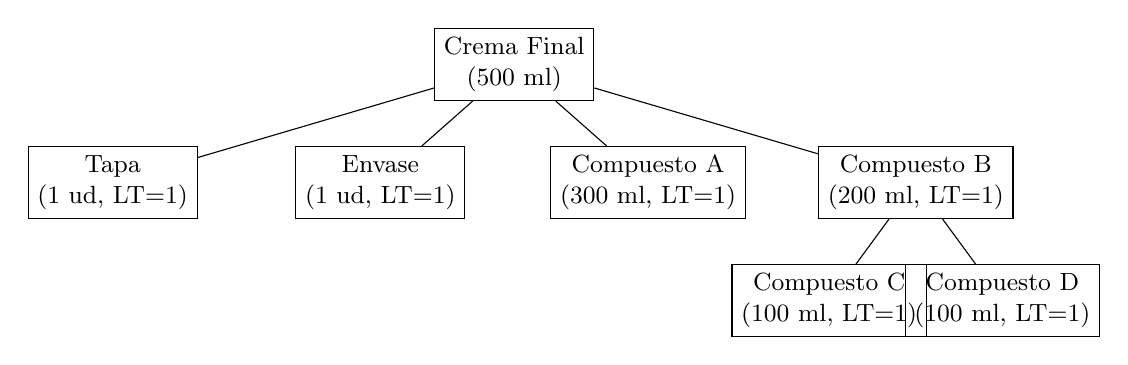
\begin{tikzpicture}[
  every node/.style={draw, font=\small, align=center},
  level 1/.style={sibling distance=34mm},
  level 2/.style={sibling distance=22mm},
  edge from parent/.style={draw, -}
]
  \node {Crema Final \\ (500 ml)}
    child {node {Tapa \\ (1 ud, LT=1)}}
    child {node {Envase \\ (1 ud, LT=1)}}
    child {node {Compuesto A \\ (300 ml, LT=1)}}
    child {node {Compuesto B \\ (200 ml, LT=1)}
      child {node {Compuesto C \\ (100 ml, LT=1)}}
      child {node {Compuesto D \\ (100 ml, LT=1)}}
    };
\end{tikzpicture}
\end{center}

\textbf{ii) Mecánica del MRP con Lote a Lote (L4L):}

Para la \textbf{Crema Final} (Producto Final):
Con $OH_0=0$, los Requerimientos Netos ($NR$) son iguales a los Requerimientos Brutos ($GR$).
Con $LT = 1$, la orden planificada ($POR$) se desfasa 1 semana:
\begin{center}\small
\begin{tabular}{@{}lccccccc@{}}
  \toprule
  Semana & 0 & 1 & 2 & 3 & 4 & 5 & 6 \\
  \midrule
  GR (Demanda) & -- & 300 & 200 & 300 & 400 & 300 & 200 \\
  POR ($L=1$)  & \textbf{300} & \textbf{200} & \textbf{300} & \textbf{400} & \textbf{300} & \textbf{200} & -- \\
  \bottomrule
\end{tabular}
\end{center}

Para el \textbf{Compuesto B} (Level 1, requerimiento = $200\text{ ml}$ por envase lanzado):
El requerimiento bruto ($GR$) de B es $200 \times POR_{\text{Crema Final}}$:
\begin{center}\small
\begin{tabular}{@{}lccccccc@{}}
  \toprule
  Semana & 0 & 1 & 2 & 3 & 4 & 5 & 6 \\
  \midrule
  GR ($200\times POR$) & 60{,}000 & 40{,}000 & 60{,}000 & 80{,}000 & 60{,}000 & 40{,}000 & -- \\
  POR ($L=1$)          & \textbf{40{,}000} & \textbf{60{,}000} & \textbf{80{,}000} & \textbf{60{,}000} & \textbf{40{,}000} & -- & -- \\
  \bottomrule
\end{tabular}
\end{center}
\textit{(Nota: Para satisfacer los 60,000 ml en la semana 0, se debe liberar la orden en la semana -1 por 60,000 ml).}

Para el \textbf{Compuesto C} (Level 2, requiere $100\text{ ml}$ por cada $200\text{ ml}$ de B, es decir, un coeficiente de $0{,}5\text{ ml}$ de C por cada ml de B):
El requerimiento bruto ($GR$) de C es $0{,}5 \times POR_B$:
\begin{center}\small
\begin{tabular}{@{}lccccccc@{}}
  \toprule
  Semana & -1 & 0 & 1 & 2 & 3 & 4 & 5 \\
  \midrule
  GR ($0{,}5\times POR$) & 30{,}000 & 20{,}000 & 30{,}000 & 40{,}000 & 30{,}000 & 20{,}000 & -- \\
  POR ($L=1$)            & \textbf{20{,}000} & \textbf{30{,}000} & \textbf{40{,}000} & \textbf{30{,}000} & \textbf{20{,}000} & -- & -- \\
  \bottomrule
\end{tabular}
\end{center}
\textit{(Nota: Para satisfacer los 30,000 ml de la semana -1, se debió liberar en la semana -2 por 30,000 ml).}

El compuesto D sigue exactamente la misma tabla que el compuesto C.

\textbf{iii) Heurística de Silver-Meal para el Compuesto C:}
Considerando demandas netas en miles de unidades (ml): $D_C = [30,\ 20,\ 30,\ 40,\ 30,\ 20]$ para las semanas W-1 a W4.
Costo de setup $S = 10$, Costo de almacenamiento $h = 1$ por unidad-semana.

\textbf{Lote a lanzar en la semana -1:}
\begin{itemize}[leftmargin=1.4em, itemsep=1pt]
  \item $k=1$ (cubre W-1): $CT(1) = 10 / 1 = 10$.
  \item $k=2$ (cubre W-1, W0): $CT(2) = \frac{10 + 1 \cdot (1) \cdot 20}{2} = 15$.
  \item Como $CT(2) > CT(1)$ ($15 > 10$), paramos. El primer lote cubre solo W-1.
  \item \textbf{Lanzamiento 1 en W-2 (por Lead-Time = 1): 30 unidades.}
\end{itemize}

\textbf{Lote a lanzar en la semana 0:}
\begin{itemize}[leftmargin=1.4em, itemsep=1pt]
  \item $k=1$ (cubre W0): $CT(1) = 10 / 1 = 10$.
  \item $k=2$ (cubre W0, W1): $CT(2) = \frac{10 + 1 \cdot (1) \cdot 30}{2} = 20$.
  \item Como $CT(2) > CT(1)$ ($20 > 10$), paramos. El lote cubre solo W0.
  \item \textbf{Lanzamiento 2 en W-1: 20 unidades.}
\end{itemize}

\textbf{Conclusión:} Debido al alto costo de almacenamiento ($h = 1$ por semana por unidad) en relación al costo de setup ($S = 10$), la regla de parada se activa inmediatamente en cada paso. Silver-Meal se comporta exactamente como Lote a Lote (L4L). El beneficio de agrupar es nulo en este caso, pues el costo por almacenar unidades para semanas posteriores supera el ahorro del costo de setup.
\end{ejercicio}


\subsection[MRP: Capacidad Limitada (I2 2022)]{MRP --- MRP Capacitado con Adelanto de Producción por Límite de Capacidad (I2 2022, Pregunta 1)}

\begin{ejercicio}{Efecto de la capacidad en la liberación de órdenes (I2 2022)}

\begin{tipprueba}{¿Cuándo usar este enfoque?}
\textbf{Identificación:} dan un producto final con su BOM, inventario disponible, lead times, y una demanda. Adicionalmente, dan una restricción de capacidad máxima de producción o ensamble por período en el nivel final y una condición de lote mínimo o producción mínima en un componente inferior. Piden completar el MRP.
\textbf{Qué aplicar:}
1) En el nivel final (nivel 0), si la demanda neta de un período supera la capacidad máxima de ensamble, se debe adelantar la producción (ensamblar en períodos previos) acumulando inventario a tiempo.
2) Esto altera las fechas de lanzamiento del producto final ($PORelease$), las cuales gatillan a su vez requerimientos brutos ($GR$) modificados en los componentes inferiores.
\end{tipprueba}

\textbf{Estructura del producto (BOM):}
\begin{center}
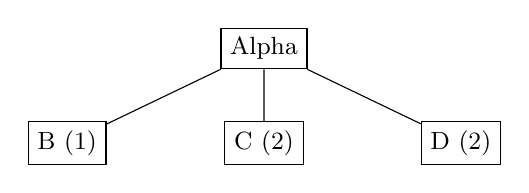
\begin{tikzpicture}[
  every node/.style={draw, font=\small},
  level distance=12mm, sibling distance=25mm,
  edge from parent/.style={draw, -}
]
  \node {Alpha}
    child {node {B (1)}}
    child {node {C (2)}}
    child {node {D (2)}};
\end{tikzpicture}
\end{center}
\textit{(Nota: El ensamble final de Alpha requiere 1 unidad de B, 2 unidades de C y 2 unidades de D).}

\textbf{Información de los componentes:}
\begin{itemize}[leftmargin=1.4em, itemsep=1pt]
  \item \textbf{Alpha} (Producto Final): $OH_0 = 10$, $LT = 1$ sem. \textbf{Capacidad máxima de ensamble} $= 27$ unidades/semana.
  \item \textbf{Componente B}: $OH_0 = 28$, $LT = 2$ sem. Loteo Lote a Lote (L4L).
  \item \textbf{Componente C}: $OH_0 = 137$, $LT = 3$ sem. Lote mínimo $= 75$ unidades.
  \item \textbf{Componente D}: $OH_0 = 100$, $LT = 1$ sem. Loteo Lote a Lote (L4L).
\end{itemize}

\textbf{Demanda externa de Alpha:} Semana 4: 50, Semana 7: 50, Semana 9: 80.

\textbf{i) Matriz MRP para Producto Final Alpha (Capacidad Máxima Ensamble = 27):}
\begin{itemize}[leftmargin=1.4em, itemsep=2pt]
  \item \textbf{Semana 4 (Demanda = 50):} Con $OH_0=10$, el requerimiento neto es $50-10 = 40$ unidades. Dado que no podemos ensamblar más de 27 por semana, debemos planificar recibir ($POR$) 27 unidades en la semana 4 y las restantes 13 en la semana 3.
  \item \textbf{Semana 7 (Demanda = 50):} Requerimiento neto es 50. Recibimos 27 unidades en la semana 7 y 23 unidades en la semana 6.
  \item \textbf{Semana 9 (Demanda = 80):} Requerimiento neto es 80. Recibimos 27 unidades en la semana 9, 27 unidades en la semana 8 y 26 unidades en la semana 7 (acumulando 3 en la semana 7 para completar).
\end{itemize}
Desfasando 1 semana por $LT=1$, obtenemos el plan de lanzamientos ($PORelease_A$):
\begin{center}\small
\begin{tabular}{@{}lcccccccccc@{}}
  \toprule
  Semana & 0 & 1 & 2 & 3 & 4 & 5 & 6 & 7 & 8 & 9 \\
  \midrule
  GR (Demanda) & -- & 0 & 0 & 0 & 50 & 0 & 0 & 50 & 0 & 80 \\
  OH           & 10 & 10 & 10 & 23 & 0 & 0 & 4 & 0 & 0 & 0 \\
  POR          & -- & 0 & 0 & 13 & 27 & 0 & 27 & 23 & 27 & 27 \\
  PORelease    & \textbf{0} & \textbf{0} & \textbf{13} & \textbf{27} & \textbf{0} & \textbf{27} & \textbf{23} & \textbf{27} & \textbf{27} & \textbf{0} \\
  \bottomrule
\end{tabular}
\end{center}

\textbf{ii) Matriz MRP para Componente B (Nivel 1, Coeficiente = 1, LT = 2):}
El requerimiento bruto ($GR$) de B es $1 \times PORelease_{Alpha}$. Con $OH_0=28$, resolvemos con L4L:
\begin{center}\small
\begin{tabular}{@{}lcccccccccc@{}}
  \toprule
  Semana & 0 & 1 & 2 & 3 & 4 & 5 & 6 & 7 & 8 & 9 \\
  \midrule
  GR           & -- & 0 & 13 & 27 & 0 & 27 & 23 & 27 & 27 & 0 \\
  OH           & 28 & 28 & 15 & 0 & 0 & 0 & 0 & 0 & 0 & 0 \\
  POR          & -- & 0 & 0 & 12 & 0 & 27 & 23 & 27 & 27 & 0 \\
  PORelease    & \textbf{0} & \textbf{12} & \textbf{0} & \textbf{27} & \textbf{23} & \textbf{27} & \textbf{27} & \textbf{0} & \textbf{0} & \textbf{0} \\
  \bottomrule
\end{tabular}
\end{center}
\textit{(Nota: El primer requerimiento neto de 12 se desfasará 2 semanas atrás, liberándose en la semana 1).}

\textbf{iii) Matriz MRP para Componente C (Nivel 1, Coeficiente = 2, LT = 3, Lote Mínimo = 75):}
El requerimiento bruto ($GR$) de C es $2 \times PORelease_{Alpha}$. Con $OH_0=137$, resolvemos considerando el lote mínimo de 75:
\begin{center}\small
\begin{tabular}{@{}lcccccccccc@{}}
  \toprule
  Semana & 0 & 1 & 2 & 3 & 4 & 5 & 6 & 7 & 8 & 9 \\
  \midrule
  GR ($2\times PORelease$) & -- & 0 & 26 & 54 & 0 & 54 & 46 & 54 & 54 & 0 \\
  OH                       & 137 & 137 & 111 & 57 & 57 & 3 & 32 & 53 & 74 & 74 \\
  POR                      & -- & 0 & 0 & 0 & 0 & 0 & 75 & 75 & 75 & 0 \\
  PORelease                & \textbf{0} & \textbf{0} & \textbf{0} & \textbf{75} & \textbf{75} & \textbf{75} & \textbf{0} & \textbf{0} & \textbf{0} & \textbf{0} \\
  \bottomrule
\end{tabular}
\end{center}
\textit{Análisis del Lote Mínimo de C:}
\begin{itemize}[leftmargin=1.4em, itemsep=1pt]
  \item En W2: $GR=26$, $OH_1=137 \implies OH_2=111$, Req Neto = 0.
  \item En W3: $GR=54$, $OH_2=111 \implies OH_3=57$, Req Neto = 0.
  \item En W4: $GR=0$, $OH_3=57 \implies OH_4=57$, Req Neto = 0.
  \item En W5: $GR=54$, $OH_4=57 \implies OH_5=3$, Req Neto = 0.
  \item En W6: $GR=46$, $OH_5=3 \implies$ Req Neto $= 43$. Se ordena el lote mínimo de \textbf{75} $\implies POR=75 \implies OH_6 = 3 + 75 - 46 = 32$. Para recibir en W6 se libera en W3 (PORel = 75).
  \item En W7: $GR=54$, $OH_6=32 \implies$ Req Neto $= 22$. Ordenamos \textbf{75} $\implies POR=75 \implies OH_7 = 32 + 75 - 54 = 53$. Se libera en W4.
  \item En W8: $GR=54$, $OH_7=53 \implies$ Req Neto $= 1$. Ordenamos \textbf{75} $\implies POR=75 \implies OH_8 = 53 + 75 - 54 = 74$. Se libera en W5.
\end{itemize}

\textbf{Conclusión:} La restricción de capacidad de ensamble obliga a nivelar el ensamblado final, adelantando la producción y suavizando las órdenes. Esto altera los momentos de liberación de componentes inferiores. Por otro lado, la restricción de lote mínimo en C genera un excedente sistemático de inventario que incrementa el stock final de la bodega.
\end{ejercicio}


\subsection[Proyectos: PERT (I2 2025)]{Administración de Proyectos --- PERT (I2 2025, Pregunta 2)}

\begin{ejercicio}{Proyecto de 6 actividades con bono/penalización (I2 2025)}

\begin{tipprueba}{¿Cuándo usar este enfoque?}
\textbf{Identificación:} dan actividades con precedentes, tiempo esperado y desviación estándar; piden ruta crítica, IC y decisión de contrato. \textbf{Qué aplicar:} forward/backward pass para la RC, $T\sim\mathcal{N}(\sum t_e, \sum\sigma^2)$ sobre la RC, y valor esperado para el bono/penalización.
\end{tipprueba}

\textbf{Datos:} A($t_e{=}13,\sigma{=}0{,}5$, sin prec.), B($12,1$), C($9,1$), D($14,2$; prec.\ A,B), E($12,1$; prec.\ B,C), F($6,0{,}4$; prec.\ E).

\textbf{i) Ruta crítica.} Caminos: A--D $= 27$; B--D $= 26$; B--E--F $= 30$; C--E--F $= 27$. La más larga es \textbf{B--E--F con $T = 30$ días}.

\textbf{ii) IC 95\% de la duración.}
\[
  \sigma_{RC}^2 = 1^2 + 1^2 + 0{,}4^2 = 2{,}16, \qquad \sigma_{RC} = \sqrt{2{,}16} = 1{,}4697
\]
\[
  IC_{95\%} = 30 \pm 1{,}96\sqrt{2{,}16} = [\,27{,}12;\ 32{,}88\,]
\]

\textbf{iii) Contrato (bono \$150 si $\le 28$; pena \$50 si $\ge 31$).}
\begin{align*}
  z_{\text{bono}} &= \tfrac{28-30}{1{,}4697} = -1{,}3608 \Rightarrow P(T\le28)=0{,}0869 \Rightarrow VE_{\text{bono}} = 0{,}0869\cdot150 = \$13{,}04\\
  z_{\text{pena}} &= \tfrac{31-30}{1{,}4697} = 0{,}6804 \Rightarrow P(T\ge31)=0{,}2483 \Rightarrow VE_{\text{pena}} = 0{,}2483\cdot50 = \$12{,}42
\end{align*}
Como $VE_{\text{bono}} > VE_{\text{pena}}$, \textbf{se acepta el contrato}.
\emph{Indiferencia:} $13{,}04 = P(T\ge t^*) \cdot 50 \Rightarrow P = 0{,}2607 \Rightarrow z = 0{,}64 \Rightarrow t^* = 30 + 0{,}64\cdot1{,}4697 \approx \mathbf{30{,}94}$ días.

\textbf{iv) Otras rutas que pueden volverse críticas.} Para cada ruta no crítica se calcula su $T$, $\sigma^2$ y la probabilidad (asumiendo independencia) de superar los 30 días: C--E--F ($\approx0{,}92\%$), A--D ($\approx3{,}43\%$), B--D ($\approx1{,}67\%$).

\textbf{Conclusión:} la ruta crítica B--E--F define el plazo; el contrato es favorable en valor esperado.
\end{ejercicio}


\subsection[Proyectos: PERT y Crashing (I2 2024)]{Proyectos --- PERT con Contratos y Crashing de Costo Mínimo (I2 2024, Pregunta 3)}

\begin{ejercicio}{Contratos e indiferencia con Crashing (I2 2024)}

\begin{tipprueba}{¿Cuándo usar este enfoque?}
\textbf{Identificación:} dan tiempos de actividades con optimista, esperado, desviación y costos. Piden: (1) ruta crítica, (2) plazo con probabilidad asimétrica, (3) evaluar aceptación de bono/multa y semanas de indiferencia, y (4) crashing de costo mínimo para acortar la ruta crítica. \textbf{Qué aplicar:} ES/EF/LS/LF, $Z$ para probabilidades, $VE = \text{Bono} \cdot P - \text{Multa} \cdot (1-p)$, y análisis marginal de costo de crashing.
\end{tipprueba}

\textbf{Datos del Proyecto:}
\begin{center}\small
\begin{tabular}{@{}ccccccc@{}}
  \toprule
  Act. & Prec. & $TE$ & $TO$ (opt.) & $\sigma$ & Costo Normal & Costo Crash (Detalles)* \\
  \midrule
  A & -- & 4 & 3 & 1{,}0 & \$4 & \$8 (1 sem, mg. \$4) \\
  B & -- & 2 & 1 & 1{,}5 & \$3 & \$6 (1 sem, mg. \$3) \\
  C & A, B & 3 & 2 & 0{,}8 & \$3 & \$6 (1 sem, mg. \$3) \\
  D & C & 2 & 1 & 2{,}0 & \$1{,}5 & \$3 (1 sem, mg. \$1{,}5) \\
  E & C & 4 & 2 & 1{,}3 & \$5 & \$10 (2 sem, mg. \$2{,}5) \\
  F & D, E & 3 & 1 & 0{,}7 & \$4 & \$8 (2 sem, mg. \$2) \\
  \bottomrule
\end{tabular}
\par\smallskip
\scriptsize *Nota: El Costo Crash nominal es el doble del Costo Normal. Se indica entre paréntesis el acortamiento máximo y su costo marginal por semana.
\end{center}

\textbf{i) Tiempos y Ruta Crítica:}
Haciendo la pasada hacia adelante y atrás obtenemos:
\begin{itemize}
  \item A: ES=0, EF=4. LS=0, LF=4. Holgura = 0.
  \item B: ES=0, EF=2. LS=2, LF=4. Holgura = 2.
  \item C (precedida por A, B): ES=4, EF=7. LS=4, LF=7. Holgura = 0.
  \item D (precedida por C): ES=7, EF=9. LS=9, LF=11. Holgura = 2.
  \item E (precedida por C): ES=7, EF=11. LS=7, LF=11. Holgura = 0.
  \item F (precedida por D, E): ES=11, EF=14. LS=11, LF=14. Holgura = 0.
\end{itemize}
La \textbf{Ruta Crítica} es \textbf{A - C - E - F} con duración $\mu_p = 14$ semanas y varianza $\sigma_p^2 = 1{,}0^2 + 0{,}8^2 + 1{,}3^2 + 0{,}7^2 = 3{,}82 \implies \sigma_p \approx 1{,}9545$ semanas.

\textbf{ii) Duración del proyecto con el doble de probabilidad de excederse que de cumplirse.}
Esto significa $P(T > X) = 2 \cdot P(T \le X) \implies 3 \cdot P(T \le X) = 1 \implies P(T \le X) = 0{,}3333$.
Buscamos en la tabla el valor de $Z$ para $0{,}3333$, el cual es $Z \approx -0{,}43$.
\[
  X = 14 - 0{,}43 \cdot 1{,}9545 = \mathbf{13{,}16}\ \text{semanas}
\]

\textbf{iii) Contrato (bono \$200 si $T \le 11$; multa \$80 si $T \ge 16$).}
\begin{itemize}
  \item Para el bono: $Z = (11 - 14)/1{,}9545 = -1{,}53 \implies P(T \le 11) = 1 - 0{,}9370 = 0{,}0630$.
  \item Para la multa: $Z = (16 - 14)/1{,}9545 = 1{,}02 \implies P(T \ge 16) = 1 - 0{,}8461 = 0{,}1539$.
  \item Valor esperado neto del contrato:
\end{itemize}
  \[
    VE = 200 \cdot (0{,}0630) - 80 \cdot (0{,}1539) = 12{,}60 - 12{,}31 = \mathbf{+\$0{,}29}
  \]
  Dado que el valor esperado es positivo, el contrato \textbf{se acepta}.
  Para la fecha de indiferencia: $P \cdot 200 = 12{,}31 \implies P(T \le X) = 0{,}0616 \implies Z \approx -1{,}54$.
  \[
    X = 14 - 1{,}54 \cdot 1{,}9545 = \mathbf{10{,}99}\ \text{semanas} \quad (\approx 11 \text{ semanas})
  \]

\textbf{iv) Crashing a costo mínimo de 3 semanas (de 14 a 11 semanas).}
Calculamos los costos de crashing por semana para cada actividad de la ruta crítica:
\begin{itemize}
  \item C: costo marginal \$3 (máximo 1 semana).
  \item F: costo marginal \$2 (máximo 2 semanas).
  \item A: costo marginal \$4 (máximo 1 semana).
  \item E: costo marginal \$2{,}5 (máximo 2 semanas).
\end{itemize}
Para reducir 3 semanas al mínimo costo:
1. Reducimos \textbf{F} en 2 semanas (Costo = \$4, la duración del proyecto baja a 12 semanas).
2. Reducimos \textbf{C} en 1 semana (Costo = \$3, la duración del proyecto baja a 11 semanas).
La ruta crítica sigue siendo A-C-E-F (duración 11 semanas, sin que se activen caminos paralelos como críticos).
El costo de crashing mínimo es de \textbf{\$7} (Costo total del proyecto = \textbf{\$27.5}).
\end{ejercicio}


\subsection[Proyectos: PERT y Tecnología (I2 2023)]{Proyectos --- PERT con Incorporación de Tecnología y Optimización (I2 2023, Pregunta B)}

\begin{ejercicio}{Evaluación de tecnología en ruta crítica y optimización (I2 2023)}

\begin{tipprueba}{¿Cuándo usar este enfoque?}
\textbf{Identificación:} dan la media $\mu$ y desviación $\sigma$ de la duración total del proyecto. Ofrecen un contrato con bono/penalización. Piden evaluar el contrato, hallar la fecha o el bono de indiferencia, y evaluar la incorporación de una tecnología que reduce la media y la desviación de una actividad en la ruta crítica, comparando el beneficio neto de la tecnología con su costo. Luego piden plantear un modelo de optimización matemática para el acortamiento.
\textbf{Qué aplicar:}
1) Estandarizar $Z = (X-\mu)/\sigma$ para probabilidades.
2) Para el cambio de varianza en PERT, restar la varianza vieja del proyecto y sumar la varianza nueva de la actividad: $Var' = Var_{\text{total}} - \sigma_{\text{vieja}}^2 + \sigma_{\text{nueva}}^2$.
3) Formular un modelo de optimización para crashing que maximice el valor esperado del contrato menos los costos de crashing.
\end{tipprueba}

\textbf{Datos iniciales del proyecto:}
\begin{itemize}[leftmargin=1.4em, itemsep=1pt]
  \item Duración esperada de la ruta crítica $\mu = 180$ días.
  \item Desviación estándar $\sigma = 12$ días $\implies$ Varianza $\sigma^2 = 144$ días$^2$.
  \item Contrato: Bono de $U\$2$ millones si $T \le 165$ días; penalidad de $U\$1$ millón si $T > 165$ días.
\end{itemize}

\textbf{i) Evaluación de Aceptación del Contrato:}
Calculamos el valor $Z$ para el umbral $X = 165$ días:
\[
  Z = \frac{165 - 180}{12} = -1{,}25
\]
De la tabla normal estándar, la probabilidad acumulada asociada es $\Phi(-1{,}25) = 1 - \Phi(1{,}25) = 1 - 0{,}8944 = 0{,}1056$.
\begin{itemize}[leftmargin=1.4em, itemsep=1pt]
  \item $P(T \le 165) = 0{,}1056$ (probabilidad de cobrar el bono).
  \item $P(T > 165) = 0{,}8944$ (probabilidad de sufrir la penalización).
\end{itemize}
El Valor Esperado neto del contrato ($VE$) es:
\[
  VE = 2 \cdot (0{,}1056) - 1 \cdot (0{,}8944) = 0{,}2112 - 0{,}8944 = -U\$0{,}6832\text{ millones} = -\$683{,}200
\]
Dado que el valor esperado es negativo, \textbf{no se acepta el contrato}.

Para ser indiferente ($VE = 0$) manteniendo la penalidad de $U\$1$ millón, despejamos el bono requerido $B$:
\[
  B \cdot (0{,}1056) - 1 \cdot (0{,}8944) = 0 \implies B = \frac{0{,}8944}{0{,}1056} \approx \mathbf{8{,}47\text{ millones}}
\]
Se requeriría un bono de \textbf{U\$8.47 millones} para estar indiferente.

\textbf{ii) Fecha de Indiferencia (Bono y Penalización Originales):}
Buscamos la probabilidad acumulada $p = P(T \le X)$ que haga $VE = 0$:
\[
  2p - 1(1 - p) = 0 \implies 3p = 1 \implies p = 0{,}3333
\]
El valor $Z$ asociado a una probabilidad acumulada de $0{,}3333$ es $Z \approx -0{,}43$. Despejamos la fecha de entrega $X$:
\[
  X = \mu + Z \cdot \sigma = 180 - 0{,}43 \cdot 12 = \mathbf{174{,}84\text{ días}}
\]
La fecha de entrega que deja indiferente al contratista es de \textbf{174.84 días}.

\textbf{iii) Evaluación de la Incorporación de Tecnología:}
Se propone una tecnología para una actividad de la ruta crítica.
\begin{itemize}[leftmargin=1.4em, itemsep=1pt]
  \item Características iniciales de la actividad: $t_0 = 20$ días, $\sigma_0 = 3$ días $\implies \sigma_0^2 = 9$ días$^2$.
  \item Impacto de la tecnología: reduce la duración en $10$ días (nueva duración $10$ días) y reduce la desviación a $1{,}5$ días $\implies \sigma_{\text{nueva}}^2 = 2{,}25$ días$^2$.
  \item Costo de la tecnología: $U\$10{,}000$.
\end{itemize}
Calculamos los nuevos parámetros del proyecto total:
\begin{align*}
  \mu' &= 180 - 10 = 170\text{ días} \\
  Var' &= Var_{\text{total}} - \sigma_0^2 + \sigma_{\text{nueva}}^2 = 144 - 9 + 2{,}25 = 137{,}25\text{ días}^2 \\
  \sigma' &= \sqrt{137{,}25} \approx 11{,}715\text{ días}
\end{align*}
\textit{(Nota: Si se usa la aproximación simplificada de la pauta de restar directo de la desviación estándar, se obtiene $\sigma' = 11.91$ días. Usamos la desviación exacta de $11{,}715$ días).}

Calculamos el nuevo $Z'$ para $X = 165$ días con la tecnología implementada:
\[
  Z' = \frac{165 - 170}{11{,}715} = -0{,}4268 \approx -0{,}43
\]
La probabilidad acumulada es $P(T \le 165) = 1 - \Phi(0{,}43) = 1 - 0{,}6664 = 0{,}3336$.
El nuevo Valor Esperado del contrato ($VE'$) es:
\[
  VE' = 2 \cdot (0{,}3336) - 1 \cdot (1 - 0{,}3336) = 0{,}6672 - 0{,}6664 = +U\$0{,}0008\text{ millones} = +U\$800
\]
\textit{(Nota: Con la aproximación de la pauta de $\sigma' = 11.91$ se obtiene $VE' = +U\$11,600$).}

Como el valor esperado pasa de $-\$683{,}200$ a $+\$800$, la tecnología genera una ganancia esperada de $U\$684{,}000$. En consecuencia, el beneficio de implementar la tecnología supera con creces su costo de $U\$10{,}000$, por lo que \textbf{sí se debe contratar la tecnología}.

\textbf{iv) Modelo de Programación Matemática para Crashing:}
Definimos:
\begin{itemize}[leftmargin=1.4em, itemsep=0pt]
  \item $x_i$: Fecha de ocurrencia del nodo $i$ del proyecto ($i=1 \dots k$, donde $k$ es el nodo final).
  \item $r_{ij}$: Días de acortamiento aplicados a la actividad que conecta el nodo $i$ con el nodo $j$.
  \item $t_{ij}$: Duración nominal de la actividad.
  \item $C_{ij}$: Costo de acortamiento unitario por día para la actividad $(i,j)$.
  \item $M_{ij}$: Acortamiento máximo permitido para la actividad $(i,j)$.
\end{itemize}

El modelo se plantea como:
\[
  \max \quad 2 \cdot \left[1 - \Phi\left(\frac{165 - x_k}{12}\right)\right] - 1 \cdot \Phi\left(\frac{165 - x_k}{12}\right) - \sum_{(i,j)} C_{ij} \cdot r_{ij}
\]
\textbf{Sujeto a:}
\begin{align*}
  x_j - x_i &\ge t_{ij} - r_{ij} && \forall (i,j) \in \text{Actividades} \\
  r_{ij} &\le M_{ij} && \forall (i,j) \in \text{Actividades} \\
  x_i, r_{ij} &\ge 0 && \forall i, j
\end{align*}
\end{ejercicio}


\subsection[Variabilidad: G/G/1 en Serie]{Variabilidad --- Colas G/G/1 en serie (Ay.\ 7, Problema 3)}

\begin{ejercicio}{Dos procesos en serie con buffer (Ayudantía 7)}

\begin{tipprueba}{¿Cuándo usar este enfoque?}
\textbf{Identificación:} procesos en serie con tiempos de proceso, CV dados y buffer. Piden throughput, WIP, tiempo de ciclo. \textbf{Qué aplicar:} Kingman ($CT_q = V\cdot U\cdot T$) para la espera en cada cola, luego sumar tiempo de proceso, y Little ($WIP = TH\cdot CT$) para el inventario.
\end{tipprueba}

\textbf{Datos:} Proceso 1: $t_e = 21$ min/trabajo $\Rightarrow \mu_1 = 60/21 = 2{,}857$/hr. Proceso 2: 3 productos/hr $\Rightarrow t_e = 20$ min. Ambos $c^2 = 1$ (exponencial). Buffer ilimitado.

\textbf{a) Throughput.} El sistema está limitado por el proceso más lento (P1, $2{,}857$/hr). En estado estacionario el TH del sistema $= $ tasa de llegada efectiva. La utilización determina la estabilidad ($\rho<1$).

\textbf{Tiempo de ciclo (Kingman por etapa):}
\[
  CT_q = \left(\frac{c_a^2 + c_e^2}{2}\right)\left(\frac{\rho}{1-\rho}\right) t_e
\]
Se suma $CT_q + t_e$ de cada etapa para el CT total. Con $WIP = TH \times CT$ (Little) se obtiene el inventario en proceso.

\textbf{b) Distribución general vs.\ exponencial.} Si los procesos tienen $c^2 < 1$ (menos variabilidad que la exponencial), el factor $V = \frac{c_a^2+c_e^2}{2}$ baja $\Rightarrow$ \textbf{menor} tiempo en cola y menor WIP. Es \textbf{mejor} tener variabilidad baja: la distribución general con $c<1$ supera a la exponencial.

\textbf{Conclusión:} la espera (y el WIP) escala con la variabilidad; reducir $c$ es la palanca clave cuando la utilización es alta.
\end{ejercicio}


\subsection[Variabilidad: M/M/1 Básico]{Variabilidad --- M/M/1 básico (Ay.\ 7, Problema 1)}

\begin{ejercicio}{Cajero único M/M/1 (Ayudantía 7)}

\begin{tipprueba}{¿Cuándo usar este enfoque?}
\textbf{Identificación:} llegadas y servicio exponenciales, un solo servidor. Piden ocio, $L_q$, $W$, throughput. \textbf{Qué aplicar:} fórmulas M/M/1 directas.
\end{tipprueba}

\textbf{Datos:} $\lambda = 10$ autos/hr; tiempo de ciclo $= 4$ min $\Rightarrow \mu = 60/4 = 15$/hr.
\begin{align*}
  \rho &= \tfrac{\lambda}{\mu} = \tfrac{10}{15} = 0{,}667 \Rightarrow \text{ocio} = 1-\rho = \mathbf{0{,}333}\ (33{,}3\%)\\
  L_q &= \tfrac{\rho^2}{1-\rho} = \tfrac{0{,}667^2}{0{,}333} = \mathbf{1{,}33}\ \text{autos en cola}\\
  W &= \tfrac{1}{\mu(1-\rho)} = \tfrac{1}{15\cdot0{,}333} = 0{,}2\ \text{hr} = \mathbf{12}\ \text{min en el sistema}\\
  \text{TH} &= \lambda = \mathbf{10}\ \text{clientes/hr (sistema estable)}
\end{align*}
\textbf{Conclusión:} el cajero está ocioso 1/3 del tiempo pero igual se forma cola por la variabilidad exponencial.
\end{ejercicio}


\subsection[Variabilidad: Capacidad (I2 2022)]{Variabilidad --- Optimización de Capacidad y Propagación en Serie (I2 2022, Pregunta 2)}

\begin{ejercicio}{Línea de comida rápida con caja registradora (I2 2022)}

\begin{tipprueba}{¿Cuándo usar este enfoque?}
\textbf{Identificación:} dan costo de espera lineal con $W_s$ y costo por unidad de capacidad. Piden tasa de servicio óptima $\mu$ (M/M/1). Luego agregan una caja registradora antes del mesón con alta variabilidad. Piden determinar el cambio en el tiempo de espera. \textbf{Qué aplicar:} optimización clásica con derivadas, Kingman y fórmula de propagación en serie ($C_d^2$).
\end{tipprueba}

\textbf{Datos:} Tasa de llegada $\lambda = 25$ clientes/hora, $C_a = 1$. Costo de espera $CE(W_s) = 10 + 1000 W_s$. Costo de servicio $= 10 \mu$ por hora. $C_s = 1$.
\begin{itemize}
  \item \textbf{a) Capacidad óptima del mesón ($\mu$):}
\end{itemize}
  Dado que $C_a = 1$ y $C_s = 1$, el mesón se comporta como un sistema M/M/1 con $W_s = 1/(\mu - 25)$.
  El costo total a minimizar es:
  \[
    CT(\mu) = 10 + \frac{1000}{\mu - 25} + 10 \mu
  \]
  Derivando con respecto a $\mu$ e igualando a cero:
  \[
    \frac{dCT}{d\mu} = -\frac{1000}{(\mu - 25)^2} + 10 = 0 \implies (\mu - 25)^2 = 100 \implies \mu = 25 + 10 = \mathbf{35}\ \text{clientes/hora}
  \]
\begin{itemize}
  \item \textbf{b) Incorporación de una caja registradora:}
\end{itemize}
  La caja tiene capacidad $\mu_1 = 50$ clientes/hora y $C_{s,1} = 2$.
  La utilización de la caja es $\rho_1 = 25/50 = 0{,}5$.
  Calculamos el coeficiente de variación de las salidas de la caja ($C_{d,1}^2$), que alimentará al mesón:
  \[
    C_{a,2}^2 \approx C_{d,1}^2 \approx \rho_1^2 \cdot C_{s,1}^2 + (1 - \rho_1)^2 \cdot C_{a,1}^2
  \]
  \[
    C_{a,2}^2 \approx 0{,}5^2 \cdot 2^2 + (1 - 0{,}5)^2 \cdot 1^2 = 0{,}25 \cdot 4 + 0{,}25 \cdot 1 = 1 + 0{,}25 = 1{,}25
  \]
  Con la llegada más variable ($C_{a,2}^2 = 1{,}25$), el mesón (ahora una cola G/G/1 con $\mu_2 = 35$, $\rho_2 = 25/35 = 0{,}714$, $C_{s,2} = 1$) tiene un tiempo de espera en cola de:
  \[
    W_{q,2} \approx \left( \frac{C_{a,2}^2 + C_{s,2}^2}{2} \right) \left( \frac{\rho_2}{1 - \rho_2} \right) \left( \frac{1}{\mu_2} \right)
  \]
  \[
    W_{q,2} \approx \left( \frac{1{,}25 + 1^2}{2} \right) \left( \frac{0{,}714}{1 - 0{,}714} \right) \left( \frac{1}{35} \right) = 1{,}125 \cdot 2{,}5 \cdot 0{,}0286 \approx \mathbf{0{,}0804}\ \text{horas} \quad (4{,}82\ \text{min})
  \]
  Sin la caja registradora, la espera en el mesón (M/M/1) era de:
  \[
    W_{q,\text{original}} = \left( \frac{1+1}{2} \right) \left( \frac{0{,}714}{1 - 0{,}714} \right) \left( \frac{1}{35} \right) \approx \mathbf{0{,}0714}\ \text{horas} \quad (4{,}29\ \text{min})
  \]

\textbf{Análisis:} El tiempo de espera en el mesón \textbf{aumenta} de 4.29 minutos a 4.82 minutos. Esto ocurre porque la caja registradora introduce una variabilidad de servicio muy alta ($C_{s,1} = 2$), la cual se propaga aguas abajo, elevando la variabilidad de las llegadas al mesón ($C_{a,2}^2 = 1{,}25 > 1$) y congestionando la cola de servicio del counter.
\end{ejercicio}

% ════════════════════════════════════════════════════════════════════════════


\subsection[Inventario: Newsvendor (I2 2023)]{Inventario --- Vendedor de Periódicos Normal vs. Uniforme (I2 2023, Pregunta A)}

\begin{ejercicio}{Vendedor de Periódicos en Tienda de Calzado (I2 2023)}

\begin{tipprueba}{¿Cuándo usar este enfoque?}
\textbf{Identificación:} se compra un ítem a costo $C$ y se vende a precio $P$, con valor de liquidación $V_s$. Piden stock óptimo bajo demanda normal y demanda uniforme. \textbf{Qué aplicar:} razón crítica $CR = C_u / (C_u + C_o)$, luego $Q^* = \mu + z \sigma$ para normal y $Q^* = a + CR \cdot (b-a)$ para uniforme.
\end{tipprueba}

\textbf{Datos:} Costo unitario $C = U\$60$, Precio de venta $P = U\$300$, Valor de liquidación $V_s = U\$47$.
\begin{itemize}[leftmargin=1.4em, itemsep=1pt]
  \item Costo de quedarse corto (Understock): $C_u = P - C = 300 - 60 = U\$240$.
  \item Costo de exceso (Overstock): $C_o = C - V_s = 60 - 47 = U\$13$.
  \item Razón Crítica ($CR$):
  \[
    CR = \frac{C_u}{C_u + C_o} = \frac{240}{240 + 13} = \frac{240}{253} \approx 0{,}9486 \quad (94{,}86\%)
  \]
\end{itemize}

\textbf{i) Demanda con distribución normal ($\mu = 300, \sigma = 40$).}
Buscamos en la tabla normal estándar el valor $Z$ tal que $\Phi(Z) = 0{,}9486$. El valor más cercano es $\Phi(1{,}64) = 0{,}9495$ y $\Phi(1{,}65) = 0{,}9505$. Usamos $Z \approx 1{,}645$.
\[
  Q^* = \mu + Z \cdot \sigma = 300 + 1{,}645 \cdot 40 = 365{,}8 \approx \mathbf{366}\ \text{pares}
\]

\textbf{ii) Demanda con distribución uniforme continua en el rango $[100, 500]$.}
La función acumulada es $F(Q) = (Q - 100)/(500 - 100)$. Igualamos a la Razón Crítica:
\[
  \frac{Q^* - 100}{400} = 0{,}9486 \implies Q^* = 100 + 0{,}9486 \cdot 400 = 100 + 379{,}44 = 479{,}44 \approx \mathbf{480}\ \text{pares}
\]
\textit{(Nota: El cálculo discreto detallado da exactamente 480 pares).}

\textbf{iii) Explicación conceptual de la diferencia.}
Aunque la demanda esperada en ambos casos es de 300 pares, la \textbf{variabilidad} (incertidumbre) en la uniforme ($\sigma \approx 115{,}5$) es mucho mayor que en la normal ($\sigma = 40$). Dado que el costo de perder una venta es muy alto ($C_u = \$240$) en relación a la pérdida por liquidar stock sobrante ($C_o = \$13$), el sistema incentiva fuertemente a sobre-comprar para cubrirse ante demandas altas. A mayor variabilidad, el riesgo de no capturar la demanda alta es mayor, por lo que se requiere comprar una cantidad mayor ($480$ vs. $366$).
\end{ejercicio}


\subsection[Bodegas: Localización (I2 2020)]{Bodegas --- Localización por Centro de Gravedad y Punto de Equilibrio (I2 2020, Pregunta III)}

\begin{ejercicio}{Ubicación de CD hoy vs. 10 años (I2 2020)}

\begin{tipprueba}{¿Cuándo usar este enfoque?}
\textbf{Identificación:} dan producción de fábricas y demanda de mercados con coordenadas geográficas $(x,y)$ para hoy y a futuro (crecimiento lineal). Proponen varias ubicaciones con costo fijo y costo variable de transporte por tonelada. Piden determinar la ubicación óptima hoy y en 10 años por Centro de Gravedad y elegir una bodega única para el horizonte evaluando costos.
\textbf{Qué aplicar:} 
1) Centro de gravedad ponderado por volumen: $C_x = \frac{\sum V_i x_i}{\sum V_i}$ y $C_y = \frac{\sum V_i y_i}{\sum V_i}$.
2) Punto de equilibrio en volumen: $CF_A + CV_A \cdot V = CF_B + CV_B \cdot V$.
3) Análisis marginal o integración de costos sobre el tiempo para evaluar la mejor ubicación única.
\end{tipprueba}

\textbf{Datos de entrada (Fábricas A, B y Mercados I, II):}
\begin{center}\small
\begin{tabular}{@{}lcccc@{}}
  \toprule
  Instalación & Vol.\ Hoy (Ton) & Vol.\ 10 años (Ton) & Coordenada $x$ & Coordenada $y$ \\
  \midrule
  Fábrica A  & 20 & 260 & 10 & 10 \\
  Fábrica B  & 70 & 140 & 40 & 20 \\
  Mercado I  & 40 & 240 & 60 & 20 \\
  Mercado II & 50 & 160 & 70 & 80 \\
  \bottomrule
\end{tabular}
\end{center}

\textbf{Ubicaciones propuestas:}
\begin{itemize}[leftmargin=1.4em, itemsep=0pt]
  \item \textbf{Lugar 1:} $(10, 60)$ con $CF_1 = \$4{,}000$ y $CV_1 = \$10$/Ton.
  \item \textbf{Lugar 2:} $(42, 29)$ con $CF_2 = \$6{,}000$ y $CV_2 = \$6$/Ton.
  \item \textbf{Lugar 3:} $(49, 35)$ con $CF_3 = \$2{,}000$ y $CV_3 = \$16$/Ton.
  \item \textbf{Lugar 4:} $(58, 20)$ con $CF_4 = \$1{,}900$ y $CV_4 = \$19$/Ton.
\end{itemize}

\textbf{i) Centro de Gravedad (CG):}
\begin{align*}
  C_x &= \frac{\sum V_i \cdot x_i}{\sum V_i}, \qquad C_y = \frac{\sum V_i \cdot y_i}{\sum V_i}
\end{align*}

\begin{itemize}[leftmargin=1.4em, itemsep=2pt]
  \item \textbf{Escenario HOY} (Volumen total $V_{\text{total}} = 180$ Ton):
    \[
      C_x^{\text{Hoy}} = \frac{20(10) + 70(40) + 40(60) + 50(70)}{180} = \frac{8{,}900}{180} \approx \mathbf{49{,}44}
    \]
    \[
      C_y^{\text{Hoy}} = \frac{20(10) + 70(20) + 40(20) + 50(80)}{180} = \frac{6{,}400}{180} \approx \mathbf{35{,}56}
    \]
    $\Rightarrow$ Centro de Gravedad Hoy = $\mathbf{(49{,}44;\ 35{,}56)}$.

  \item \textbf{Escenario 10 AÑOS} (Volumen total $V_{\text{total}} = 800$ Ton):
    \[
      C_x^{\text{10a}} = \frac{260(10) + 140(40) + 240(60) + 160(70)}{800} = \frac{33{,}800}{800} \approx \mathbf{42{,}25}
    \]
    \[
      C_y^{\text{10a}} = \frac{260(10) + 140(20) + 240(20) + 160(80)}{800} = \frac{23{,}000}{800} \approx \mathbf{28{,}75}
    \]
    $\Rightarrow$ Centro de Gravedad 10 años = $\mathbf{(42{,}25;\ 28{,}75)}$.
\end{itemize}

\textbf{ii) Comparación de ubicaciones sugeridas:}
\begin{itemize}[leftmargin=1.4em, itemsep=2pt]
  \item \textbf{Para Hoy:} El CG es $(49{,}44;\ 35{,}56)$. El \textbf{Lugar 3} $(49, 35)$ es la alternativa real más cercana.
    \[
      \text{Costo Hoy (Lugar 3)} = 2{,}000 + 16(180) = \mathbf{\$4{,}880}
    \]
  \item \textbf{Para 10 años:} El CG es $(42{,}25;\ 28{,}75)$. El \textbf{Lugar 2} $(42, 29)$ es la alternativa real más cercana.
    \[
      \text{Costo 10a (Lugar 2)} = 6{,}000 + 6(800) = \mathbf{\$10{,}800}
    \]
\end{itemize}

\textbf{iii) Elección de bodega única para los próximos 10 años:}
El crecimiento de volumen es lineal (de 180 Ton en $t=0$ a 800 Ton en $t=10$). El volumen en el año $t$ es:
\[
  V(t) = 180 + 62t \qquad \forall t\in[0,10]
\]
Evaluamos el punto de equilibrio entre el Lugar 3 (bajo costo fijo, alto variable) y el Lugar 2 (alto costo fijo, bajo variable):
\begin{align*}
  CF_3 + CV_3 \cdot V &= CF_2 + CV_2 \cdot V \\
  \implies 2{,}000 + 16V &= 6{,}000 + 6V \implies 10V = 4{,}000 \implies \mathbf{V^* = 400\text{ Ton}}
\end{align*}
\begin{itemize}[leftmargin=1.4em, itemsep=2pt]
  \item Si $V(t) < 400$ Ton $\Rightarrow$ Conviene Lugar 3. Esto ocurre desde $t=0$ hasta $t = (400-180)/62 \approx 3{,}55$ años.
  \item Si $V(t) > 400$ Ton $\Rightarrow$ Conviene Lugar 2. Esto ocurre desde $t=3{,}55$ hasta $t=10$ años.
\end{itemize}
Dado que el crecimiento es lineal, podemos comparar los ahorros acumulados mediante el análisis geométrico de las áreas de costo sobre el rango de volumen $[180, 800]$:
\begin{itemize}[leftmargin=1.4em, itemsep=2pt]
  \item \textbf{Beneficio de Lugar 3 sobre Lugar 2 (cuando $V \in [180, 400]$):}
    La diferencia máxima de costo es en $V=180$, donde $\text{Costo}_2(180) - \text{Costo}_3(180) = (6{,}000+6\cdot180) - (2{,}000+16\cdot180) = 7{,}080 - 4{,}880 = \$2{,}200$.
    El beneficio acumulado (área de la diferencia) es:
    \[
      \text{Área 3} = \frac{(400 - 180) \times 2{,}200}{2} = \mathbf{\$242{,}000\text{ Ton-USD}}
    \]
  \item \textbf{Beneficio de Lugar 2 sobre Lugar 3 (cuando $V \in [400, 800]$):}
    La diferencia máxima de costo es en $V=800$, donde $\text{Costo}_3(800) - \text{Costo}_2(800) = (2{,}000+16\cdot800) - (6{,}000+6\cdot800) = 14{,}800 - 10{,}800 = \$4{,}000$.
    El beneficio acumulado es:
    \[
      \text{Área 2} = \frac{(800 - 400) \times 4{,}000}{2} = \mathbf{\$800{,}000\text{ Ton-USD}}
    \]
\end{itemize}
Dado que el área de beneficio para el Lugar 2 ($\$800{,}000$) es mucho mayor que para el Lugar 3 ($\$242{,}000$), la bodega única óptima para el horizonte de 10 años es el \textbf{Lugar 2}.

\textbf{Conclusión:} A largo plazo, el volumen acumulado justifica el mayor costo fijo del Lugar 2 para beneficiarse de su menor costo variable de transporte.
\end{ejercicio}


